\section{Robustness Without the Noise Reference}
\label{app:robust-z}

\begin{table}[t]
\centering
\caption{Robustness check of the all-datasets rows of Table~\ref{tab:summary}: the same fits with each outcome replaced by
its robust $z$ score, $(x-\mathrm{median})/(\mathrm{IQR}/1.349)$ over models, computed within each dataset unit, so that no noise
reference is involved and each unit has the same spread of model scores. Coefficient (SE); reference: Standard LLM of the same size and perplexity. $^{*}p<.05$, $^{**}p<.01$, $^{***}p<.001$.}
\label{tab:summary-z}
\setlength{\tabcolsep}{3pt}
\resizebox{\linewidth}{!}{%
\begin{tabular}{@{}lcccccc@{}}
\toprule
 & Memory $\beta_M$ & Data $\beta_D$ & $M\times D$ $\beta_{MD}$ & $\log_{10}$ params $\beta_S$ & $\log_{10}$ PPL $\beta_P$ & C-BabyLM vs.\ LLM \\
\midrule
\multicolumn{7}{@{}l}{\textit{All datasets \quad (16 reading measures; 8 neural datasets)}} \\
\quad Behavior & $+.293^{*}$ (.126) & $+.480^{*}$ (.178) & $-.480^{*}$ (.189) & $-.447^{***}$ (.043) & $-.275^{***}$ (.042) & $+.294^{*}$ (.136) \\
\quad Brain & $-.459^{*}$ (.220) & $-.305$ (.289) & $+.285$ (.318) & $+.426^{***}$ (.096) & $-.008$ (.110) & $-.479$ (.243) \\
\bottomrule
\end{tabular}}
\end{table}


The split-half reference rescales each dataset unit by a constant. It sets the weight of a unit in the medians and the scale of the coefficients, but it is not an upper bound for multichannel datasets (Appendix~\ref{app:rsa-ceilings}). Table~\ref{tab:summary-z} repeats the all-datasets fits of Table~\ref{tab:summary} with an outcome that uses no reference: the robust $z$ score of the raw $\Delta\ell$ over models, computed within each dataset unit. Coefficients are then in standard deviations of model scores.

The behavioral advantage of both constraints remains (memory $+.29$, data $+.48$, Constrained-BabyLM $+.29$, all $p<.05$, negative interaction), and so does the size dissociation. On the brain side, the memory constraint is associated with lower similarity ($-.46$, $p=.041$), the data constraint is not reliable, and the Constrained-BabyLM contrast is borderline ($-.48$, $p=.052$). No constraint is associated with higher brain similarity under either outcome.

\section{Natural Stories and Podcast Alone}
\label{app:two-datasets}

\begin{figure}[h]
\centering
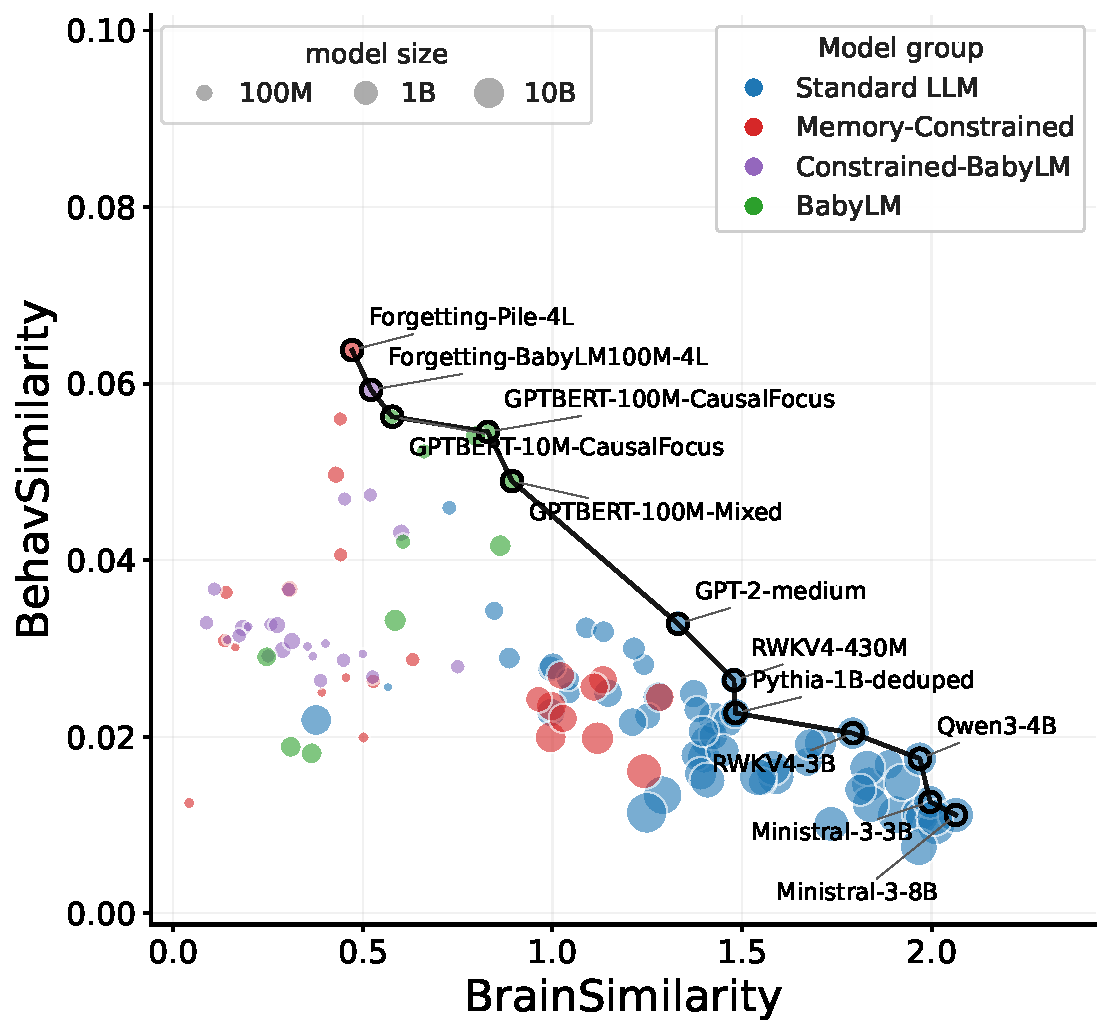
\includegraphics[width=.62\linewidth]{figures/rsa_ns_podcast_pareto.pdf}
\caption{Brain similarity (Podcast ECoG, language network) against behavioral similarity (Natural Stories self-paced reading) for 118 models, each divided by the split-half reference of its dataset. Layout as in Figure~\ref{fig:method}B.}
\label{fig:ns-podcast}
\end{figure}

\begin{table}[t]
\centering
\small
\setlength{\tabcolsep}{4pt}
\caption{Two-dataset matched-scale regression: Natural Stories self-paced reading (118 models) and Podcast ECoG, language
network (116 models); one row per model, OLS with family-clustered standard errors. Outcome: score divided by the split-half
reference. Coefficient (SE); reference: Standard LLM. $^{*}p<.05$, $^{**}p<.01$, $^{***}p<.001$.}
\label{tab:rsa-two}
\resizebox{\linewidth}{!}{%
\begin{tabular}{lcc}
\toprule
 & Behavior & Brain \\
\midrule
Memory constraint $\beta_M$ & $+.006$ (.004) & $-.300^{***}$ (.058) \\
Data constraint $\beta_D$ & $+.014^{***}$ (.002) & $-.315^{***}$ (.050) \\
Interaction $\beta_{MD}$ & $-.010^{***}$ (.002) & $+.316^{***}$ (.062) \\
$\log_{10}$ parameters $\beta_S$ & $-.013^{***}$ (.002) & $+.211^{**}$ (.078) \\
$\log_{10}$ perplexity $\beta_P$ & $-.008^{**}$ (.002) & $-.249^{**}$ (.079) \\
\bottomrule
\end{tabular}}
\end{table}


Natural Stories and Podcast are the two naturalistic datasets with every word pair in the RDM (about 10,200 and 5,100 words), and the two used for the syntactic-load bins. On these two alone (Figure~\ref{fig:ns-podcast}), the front runs from Forgetting-Pile-4L, a four-layer forgetting-attention model, through Forgetting-BabyLM100M-4L and three GPT-BERT BabyLM models, to Standard LLMs (GPT-2-medium, RWKV-4, Pythia-1B, Qwen3-4B, Ministral-3-3B and 8B). At matched scale (Table~\ref{tab:rsa-two}), the data constraint is associated with higher behavioral similarity ($+.014$, $p<.001$), the memory constraint is positive but not reliable, and both constraints are associated with lower brain similarity (about $-.30$ each, $p<.001$).

\section{Multiple-Demand Network}
\label{app:md}

\paragraph{Units.} \emph{Pereira}: voxels of the MD atlas released with the dataset \citep{pereira2018toward}, concatenated over the participants of each passage set, as for the language atlas. \emph{Podcast}: all electrodes were re-extracted; an electrode is assigned to the MD network if it is word-responsive, not in one of the five language regions, and within 10\,mm of a voxel with probability $\geq.1$ in a probabilistic MD map from an MD localizer in 691 participants, distributed with the atlases of \citet{lipkin2022probabilistic}. \emph{Tuckute}: the mean response of the functionally localized MD regions of both hemispheres, against the mean of the left-hemisphere language regions; both are group-level item means. All other choices (model RDM, confounds, folds) are those of the main analysis.

\paragraph{Why ranks.} MD split-half references are 3--15 times smaller than the language references (Pereira: $\Delta\ell$ $.00048$ and $.00053$ for the two passage sets, about a third of the language reference) and noisy, so normalized MD scores reach 5 to 60 times the reference. The outcome of Table~\ref{tab:summary} is therefore the percentile rank of each model's raw $\Delta\ell$ within each dataset and network, which uses no reference and gives each dataset the same weight.

\begin{table}[t]
\centering
\caption{Language vs.\ multiple-demand network per dataset: matched-scale regression (Equation~\ref{eq:group} without random
effects) of the percentile rank of the raw $\Delta\ell$ among the 118 models (as in Table~\ref{tab:summary}), one row per model, lineage random intercept (REML, Satterthwaite $t$-tests). Coefficient (SE);
reference: Standard LLM. $^{*}p<.05$, $^{**}p<.01$, $^{***}p<.001$.}
\label{tab:md-datasets}
\resizebox{\linewidth}{!}{%
\begin{tabular}{@{}lcccccc@{}}
\toprule
 & \multicolumn{2}{c}{Pereira (fMRI)} & \multicolumn{2}{c}{Podcast (ECoG)} & \multicolumn{2}{c}{Tuckute (fMRI)} \\
\cmidrule(lr){2-3}\cmidrule(lr){4-5}\cmidrule(lr){6-7}
 & Language & MD & Language & MD & Language & MD \\
\midrule
Memory constraint $\beta_M$ & $-.009$ (.047) & $-.003$ (.046) & $-.111^{*}$ (.045) & $-.130^{*}$ (.058) & $-.120$ (.077) & $-.084$ (.110) \\
Data constraint $\beta_D$ & $-.100$ (.060) & $-.098$ (.059) & $-.163^{*}$ (.060) & $-.142$ (.076) & $+.027$ (.102) & $+.051$ (.149) \\
Interaction $\beta_{MD}$ & $+.072$ (.066) & $+.071$ (.064) & $+.150^{*}$ (.064) & $+.115$ (.082) & $-.001$ (.111) & $+.105$ (.161) \\
$\log_{10}$ parameters $\beta_S$ & $+.108^{***}$ (.023) & $+.111^{***}$ (.022) & $+.075^{***}$ (.021) & $+.184^{***}$ (.029) & $+.208^{***}$ (.031) & $-.055$ (.041) \\
$\log_{10}$ perplexity $\beta_P$ & $-.175^{***}$ (.033) & $-.179^{***}$ (.032) & $-.160^{***}$ (.031) & $+.021$ (.042) & $+.035$ (.039) & $-.073$ (.054) \\
C-BabyLM vs.\ LLM & $-.037$ (.052) & $-.029$ (.050) & $-.124^{*}$ (.050) & $-.158^{*}$ (.066) & $-.094$ (.087) & $+.072$ (.123) \\
\bottomrule
\end{tabular}}
\end{table}


\paragraph{Per dataset.} Table~\ref{tab:md-datasets} fits each dataset separately. In Pereira and Podcast, where models do predict the MD RDM, the constraint coefficients are nearly the same on the two networks (Pereira data $-.100$ and $-.098$, both $p=.10$; Podcast memory $-.111$ and $-.130$, data $-.163$ and $-.142$, Constrained-BabyLM $-.124$ and $-.158$). In Tuckute, where no model predicts the MD response above the length-and-frequency baseline, no coefficient is reliable on either network, and the Constrained-BabyLM contrast is positive on the MD network ($+.072$, $p=.56$). The smaller penalty on the MD network in the pooled fit of Table~\ref{tab:summary} therefore reflects Tuckute's noise-level MD scores rather than a better match of constrained models to the MD network.
